\chapter{Pengenalan Cloud Computing dan Infrastruktur Pengembangan Aplikasi Berbasis Node.js}

\section{Apa itu Cloud Computing?}

Cloud Computing, \index{Cloud Computing} atau sering diterjemahkan sebagai ``Komputasi Awan'' dalam bahasa Indonesia mempunyai berbagai definisi:\index{Cloud Computing!Definisi}
\begin{itemize}
  \item \textbf{Wikipedia}: penggunaan sumber daya komputasi (peranti keras dan peranti lunak) yang berfungsi untuk memberikan layanan melalui suatu jaringan (pada umumnya Internet)\footnote{\url{http://en.wikipedia.org/wiki/Cloud_computing}}.
  \item \textbf{NIST\footnote{The National Institute of Standards and Technology}}: model yang memungkinkan akses jaringan ubiquitous (dari mana saja), nyaman, on-demand (saat ada permintaan) ke sekumpulan sumber daya komputasi yang dikonfigurasi untuk berbagi (jaringan, server, penyimpanan, dan berbagai layanan lain) yang dapat dengan cepat ditetapkan dan dirilis dengan usaha yang minimal dari manajemen ataupun interaksi dengan penyedia layanan\footnote{\url{http://csrc.nist.gov/publications/PubsSPs.html\#800-145}}.
\end{itemize}

Jika diwujudkan secara visual, Cloud Computing bisa dilihat pada Gambar~\ref{fig:ccsam}\footnote{Gambar dibuat oleh Sam Johnston, diambil dari \url{http://en.wikipedia.org/w/index.php?title=File:Cloud_computing.svg&page=1}}

  \begin{figure}[t]
    \begin{center}
      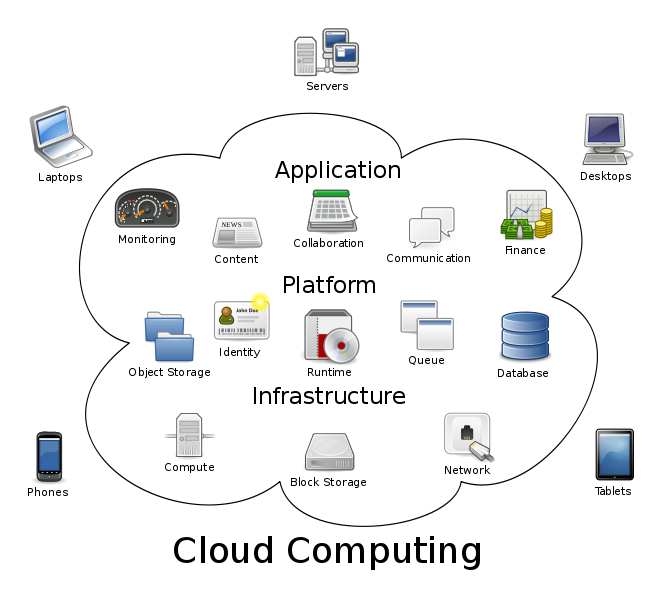
\includegraphics[scale=0.5]{images/662px-Cloud_computing.png}
    \end{center}
    \caption{Model Cloud Computing}
    \label{fig:ccsam}
  \end{figure}

\section{Karakteristik Cloud Computing}

Menurut NIST, ada beberapa karakteristik dari Cloud Computing:\index{Cloud Computing!Karakteristik}
\begin{itemize}
  \item \textbf{On-demand self-service}: layanan bisa diperoleh pada saat diminta, tanpa intervensi atau interaksi manusia di sisi penyedia jasa. 
  \item \textbf{Broad network access}: tersedia melalui jaringan dengan berbagai peranti yang umum (komputer, tablet, HP, dan lain-lain)
  \item \textbf{Resource pooling}: sumber daya komputasi dari penyedia jasa terkumpul untuk melayani.
  \item \textbf{Rapid elasticity}: skalabilitas.
  \item \textbf{Measured service}: penggunaan sumber daya bisa diukur, di-monitor, dikendalikan, dan dilaporkan.
\end{itemize}

Karakteristik lain yang tidak kalah penting adalah \textit{multitenancy}. \textit{Multitenancy} merupakan suatu prinsip dalam arsitektur software. Pada arsitektur tersebut, satu instan dari software berjalan pada server, melayani banyak organisasi klien. Aplikasi dirancang untuk mempartisi data dan konfigurasinya secara virtual dan setiap organisasi klien tersebut bekerja dengan instan aplikasi virtual tersebut\footnote{\url{http://en.wikipedia.org/wiki/Multitenancy}}. \index{Multitenancy}

\section{\textit{Public} dan \textit{Private} Cloud Computing}

\index{Cloud Computing!Private}Cloud Computing bisa dibangun untuk keperluan pribadi suatu organisasi dan (secara legal) hanya bisa diakses oleh organisasi yang bersangkutan. Tipe tersebut dikenal dengan \textit{Private Cloud Computing}. \index{Cloud Computing!Public}Sementara itu, jika sumber daya Cloud Computing bisa diakses oleh publik (dengan hak akses yang sesuai), maka model tersebut dikenal sebagai \textit{Public Cloud Computing}. Pembahasan di buku ini adalah pembahasan tentang \textit{Public Cloud Computing} dan semua referensi tentang Cloud Computing di buku ini akan menunjuk pada \textit{Public Cloud Computing} kecuali dinyatakan lain.

\section{Model Layanan Cloud Computing}

\index{Cloud Computing!Model layanan}Model layanan pada Cloud Computing akan berkembang sesuai kebutuhan konsumen serta inovasi dari berbagai penyedia layanan. Saat ini, pada umumnya, ada tiga model layanan:
\begin{itemize}
  \item \textbf{SaaS} (\textit{Software as a Service}): layanan berupa aplikasi yang ditempatkan pada infrastruktur penyedia layanan, siap digunakan oleh konsumen.
  \item \textbf{PaaS} (\textit{Platform as a Service}): menyediakan layanan ke konsumen berupa platform untuk men-deploy aplikasi.
  \item \textbf{IaaS} (\textit{Infrastructure as a Service}): menyediakan layanan ke konsumen berupa berbagai sumber daya komputasi (pemrosesam, penyimpanan, jaringan, dan sumber daya fundamental lainnya).
\end{itemize}

Meski sampai saat ini, umumnya terdapat tiga model tersebut, beberapa model kelihatannya sudah mulai muncul, misalnya STaaS (\textit{Storage as a Service}), SECaaS (\textit{Security as a Service}), DaaS (\textit{Data as a Service}), TEaaS (\textit{Test Environment as a Service}), \textit{Desktop Virtualization}, APIaaS (\textit{API as a Service}).

\section{Pengembangan Aplikasi di Cloud Computing}

Pada umumnya, para pengembang aplikasi di Cloud Computing juga menggunakan pendekatan \textit{Agile Software Development} yang berbasis pada pengembangan secara iteratif untuk setiap \textit{milestone} (dalam iterasi analisis-desain-\textit{coding-testing-debugging}) mulai dari \textit{milestone} paling awal sampai software dirilis. Perbedaan paling mendasar hanyalah pada platform yang digunakan untuk \textit{deployment}, peranti pengembangan yang digunakan, serta utilitas untuk mengelola aplikasi yang di-\textit{deploy} pada instan di cloud.

Pengembangan aplikasi di Cloud Computing akan melibatkan peranti pengembang yang didukung oleh infrastruktur Cloud. Kita akan memerlukan PaaS untuk keperluan ini. Pada dasarnya pengembangan aplikasi akan meliputi siklus berikut:

\begin{itemize}
  \item \textit{Coding}
  \item Test di komputer lokal
  \item Upload ke server (dalam Cloud Computing, proses ini diistilahkan dengan ``\textit{push}''
  \item Edit - push
\end{itemize}

Jika pengembangan aplikasi dilakukan oleh tim, maka perlu adanya software untuk \textit{version control}, misalnya Git, mercurial, dan lain-lain. Setelah itu, aktivitas yang dilakukan biasanya terpusat pada \textit{push} (untuk mengupload instan dari aplikasi ke server) dan \textit{pull} (untuk mengambil instan aplikasi dari server).

\section{Node.js dan Cloud Computing}

\index{Node.js}Node.js merupakan salah satu peranti pengembang yang bisa digunakan untuk membuat aplikasi berbasis Cloud. Node.js dikembangkan dari \textit{engine} JavaScript yang dibuat oleh Google untuk browser \textit{Chrome / Chromium} (V8). Dengan menggunakan Node.js, semua pengembangan akan dilakukan menggunakan JavaScript, baik pada sisi klien maupun server. Node.js dibuat pertama kali oleh Ryan Dahl (twitter.com/ryah) dan sampai saat ini dikembangkan oleh komunitas sebagai software bebas dengan pendanaan utama dari Joyent, perusahaan tempat Ryan Dahl bekerja.

\section{Layanan Hosting Aplikasi: CloudFoundry}

\index{CloudFoundry}Saat ini, mulai banyak penyedia layanan Cloud yang mendukung Node.js, diantaranya adalah CloudFoundry (\url{http://www.cloudfoundry.com}, selanjutnya akan kita sebut dengan CF). Buku ini akan menggunakan fasilitas dari CF. Daftar lengkap dari penyedia infrastruktur Node.js bisa dilihat pada \url{https://github.com/joyent/node/wiki/Node-Hosting}.\index{Node.js!Hosting}

\subsection{Pendaftaran}

Untuk menggunakan fasilitas dari CF, kita akan mendaftar lebih dahulu di URL \url{https://mycloudfoundry.com/signup} sepert yang terlihat pada Gambar~\ref{fig:cfsignup}.

\begin{figure}[t]
    \begin{center}
      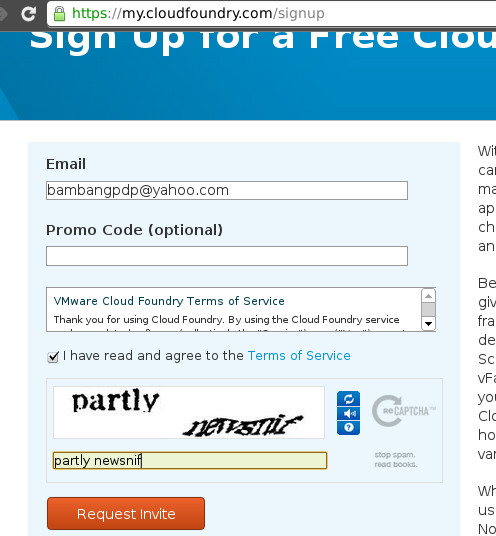
\includegraphics[scale=0.5]{images/cf-signup.jpg}
    \end{center}
    \caption{Pendaftaran di CF}
    \label{fig:cfsignup}
  \end{figure}

Setelah itu, CF akan mengirimkan pemberitahuan bahwa proses pendaftaran selesai seperti di Gambar~\ref{fig:cfsignuphasil}. \textit{Credentials} atau informasi tentang akun kita di CF akan dikirimkan ke e-mail kita seperti pada Gambar~\ref{fig:cfsignupapproved}.
 
  \begin{figure}
    \begin{center}
      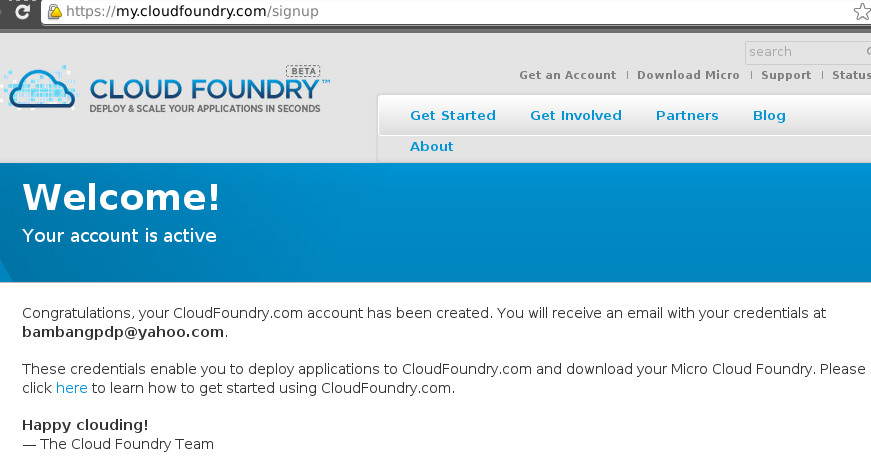
\includegraphics[scale=0.5]{images/cf-signup-hasil.jpg}
    \end{center}
    \caption{Hasil proses pendaftaran di CF}
    \label{fig:cfsignuphasil}
  \end{figure}

  \begin{figure}[t]
    \begin{center}
      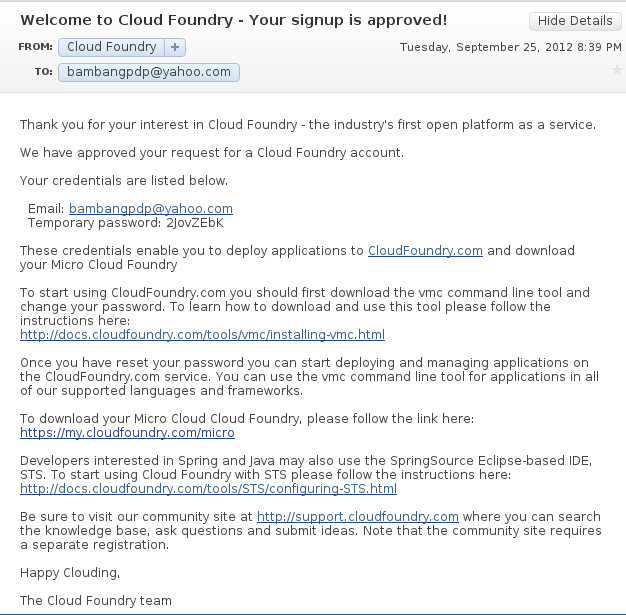
\includegraphics[scale=0.5]{images/cf-signup-approved.jpg}
    \end{center}
    \caption{E-mail persetujuan dan pemberitahuan \textit{credentials}}
    \label{fig:cfsignupapproved}
  \end{figure}

\subsection{Instalasi \textit{Command Line Utilities}}

\index{CloudFoundry!vmc}\textit{Command Line Utilities / CLU)} adalah software yang dijalankan melalui shell / \textit{command line / command prompt}. CLU untuk CF ini dibuat dengan menggunakan Ruby dan didistribusikan dalam bentuk \textit{gem} sehingga untuk instalasi ini diperlukan ruby dan rubygem. Berikut adalah perintah untuk instalasi vmc (CLU dari CF).

\lstset{language=bash,caption=Instalasi vmc}
\begin{lstlisting}
$ gem search vmc --remote | grep "\bvmc\s" 
vmc (0.3.21) 
$ gem install vmc 
Fetching: multi_json-1.3.6.gem (100%) 
Fetching: cfoundry-0.3.34.gem (100%) 
Fetching: vmc-0.3.21.gem (100%) 
Successfully installed multi_json-1.3.6 
Successfully installed cfoundry-0.3.34 
Successfully installed vmc-0.3.21 
3 gems installed 
Installing ri documentation for multi_json-1.3.6... 
Installing ri documentation for cfoundry-0.3.34... 
Installing ri documentation for vmc-0.3.21... 
Installing RDoc documentation for multi_json-1.3.6... 
Installing RDoc documentation for cfoundry-0.3.34... 
Installing RDoc documentation for vmc-0.3.21... 
$
\end{lstlisting}

Hasil dari instalasi tersebut adalah sebagai berikut:

\lstset{language=bash,caption=Hasil gem yang terinstall}
\begin{lstlisting}
$ gem list 

*** LOCAL GEMS *** 

addressable (2.2.8) 
af (0.3.18.6) 
bigdecimal (1.1.0) 
cfoundry (0.3.34) 
interact (0.4.8) 
io-console (0.3) 
json (1.5.4) 
json_pure (1.6.7) 
mime-types (1.19) 
minitest (2.5.1) 
multi_json (1.3.6) 
rake (0.9.2.2) 
rb-readline (0.4.2) 
rdoc (3.9.4) 
rest-client (1.6.7) 
rubyzip (0.9.9) 
terminal-table (1.4.5) 
uuidtools (2.1.3) 
vmc (0.3.21) 
$ 
\end{lstlisting}

Setelah itu, tambahkan baris berikut di \textit{\$HOME/.bashrc} (catatan: "/home/bpdp/" adalah direktori \$HOME saya, silahkan sesuaikan dengan tempat anda):

\lstset{language=bash,caption=Mengaktifkan direktori "bin" hasil instalasi gem}
\begin{lstlisting}
export PATH=$PATH:/home/bpdp/.gem/ruby/1.9.1/bin
\end{lstlisting}

Periksa dengan menjalankan opsi help dari vmc:

\lstset{language=bash,caption=Hasil opsi help dari vmc}
\begin{lstlisting}
$ vmc help 

Usage: vmc [options] command [<args>] [command_options] 
Try 'vmc help [command]' or 'vmc help options' for more information. 

Currently available vmc commands are: 

  Getting Started 
    target [url]                                 Reports current target or sets a new target 
    login  [email] [--email, --passwd]           Login 
    info                                         System and account information 

  Applications 
    apps                                         List deployed applications 

  Application Creation 
    push [appname]                               Create, push, map, and start a new application 
    push [appname] --path                        Push application from specified path 
    push [appname] --url                         Set the url for the application 
    push [appname] --instances <N>               Set the expected number <N> of instances 
    push [appname] --mem M                       Set the memory reservation for the application 
    push [appname] --runtime RUNTIME             Set the runtime to use for the application 
    push [appname] --debug [MODE]                Push application and start in a debug mode 
    push [appname] --no-start                    Do not auto-start the application 

  Application Operations 
    start <appname> [--debug [MODE]]             Start the application 
    stop  <appname>                              Stop the application 
    restart <appname> [--debug [MODE]]           Restart the application 
    delete <appname>                             Delete the application 

  Application Updates 
    update <appname> [--path,--debug [MODE]]     Update the application bits 
    mem <appname> [memsize]                      Update the memory reservation for an application 
    map <appname> <url>                          Register the application to the url 
    unmap <appname> <url>                        Unregister the application from the url 
    instances <appname> <num|delta>              Scale the application instances up or down 

  Application Information 
    crashes <appname>                            List recent application crashes 
    crashlogs <appname>                          Display log information for crashed applications 
    logs <appname> [--all]                       Display log information for the application 
    files <appname> [path] [--all]               Display directory listing or file download for [path] 
    stats <appname>                              Display resource usage for the application 
    instances <appname>                          List application instances 

  Application Environment 
    env <appname>                                List application environment variables 
    env-add <appname> <variable[=]value>         Add an environment variable to an application 
    env-del <appname> <variable>                 Delete an environment variable to an application 

  Services 
    services                                     Lists of services available and provisioned 
    create-service <service> [--name,--bind]     Create a provisioned service 
    create-service <service> <name>              Create a provisioned service and assign it <name> 
    create-service <service> <name> <app>        Create a provisioned service and assign it <name>, and bind to <app> 
    delete-service [servicename]                 Delete a provisioned service 
    bind-service <servicename> <appname>         Bind a service to an application 
    unbind-service <servicename> <appname>       Unbind service from the application 
    clone-services <src-app> <dest-app>          Clone service bindings from <src-app> application to <dest-app> 
    tunnel <servicename> [--port]                Create a local tunnel to a service 
    tunnel <servicename> <clientcmd>             Create a local tunnel to a service and start a local client 

  Administration 
    user                                         Display user account information 
    passwd                                       Change the password for the current user 
    logout                                       Logs current user out of the target system 
    add-user [--email, --passwd]                 Register a new user (requires admin privileges) 
    delete-user <user>                           Delete a user and all apps and services (requires admin privileges) 

  System 
    runtimes                                     Display the supported runtimes of the target system 
    frameworks                                   Display the recognized frameworks of the target system 

  Micro Cloud Foundry 
    micro status                                 Display Micro Cloud Foundry VM status 
    micro offline                                Configure Micro Cloud Foundry VM for offline mode 
    micro online                                 Configure Micro Cloud Foundry VM for online mode 
      [--vmx file]                               Path to micro.vmx 
      [--vmrun executable]                       Path to vmrun executable 
      [--password cleartext]                     Cleartext password for guest VM vcap user 
      [--save]                                   Save cleartext password in ~/.vmc_micro 

  Misc 
    aliases                                      List aliases 
    alias <alias[=]command>                      Create an alias for a command 
    unalias <alias>                              Remove an alias 
    targets                                      List known targets and associated authorization tokens 

  Help 
    help [command]                               Get general help or help on a specific command 
    help options                                 Get help on available options 

$ 
\end{lstlisting}

\subsection{Konfigurasi di Server Cloud}

Pada dasarnya, yang diperlukan hanyalah mengubah target ke server cloud dari CF dan kemudian mengubah password.

\lstset{language=bash,caption=Mengubah target server}
\begin{lstlisting}
$ vmc target 

[http://api.vcap.me] 

$ vmc target api.cloudfoundry.com 
Successfully targeted to [http://api.cloudfoundry.com] 

$ vmc target 
 
[http://api.cloudfoundry.com] 

$ 
\end{lstlisting}

Setelah itu, setiap kali kita akan melakukan berbagai proses yang melibatkan server ini, kita harus melakukan proses login terlebih dahulu:

\lstset{language=bash,caption=Login ke server}
\begin{lstlisting}
$ vmc login 
Attempting login to [http://api.cloudfoundry.com] 
Email: bambangpdp@yahoo.com 
Password: ******** 
Successfully logged into [http://api.cloudfoundry.com] 

$ vmc info 

VMware's Cloud Application Platform 
For support visit http://support.cloudfoundry.com 

Target:   http://api.cloudfoundry.com (v0.999) 
Client:   v0.3.21 

User:     bambangpdp@yahoo.com 
Usage:    Memory   (0B of 2.0G total) 
          Services (0 of 16 total) 
          Apps     (0 of 20 total) 

$ vmc runtimes 

+--------+-------------+-----------+ 
| Name   | Description | Version   | 
+--------+-------------+-----------+ 
| java   | Java 6      | 1.6       | 
| java7  | Java 7      | 1.7       | 
| node   | Node.js     | 0.4.12    | 
| node06 | Node.js     | 0.6.8     | 
| node08 | Node.js     | 0.8.2     | 
| ruby18 | Ruby 1.8    | 1.8.7     | 
| ruby19 | Ruby 1.9    | 1.9.2p180 | 
+--------+-------------+-----------+ 

$ 
\end{lstlisting}

Untuk mengubah password:

\lstset{language=bash,caption=Mengubah password server}
\begin{lstlisting}
$ vmc passwd 
Changing password for 'bambangpdp@yahoo.com' 
New Password: ******** 
Verify Password: ******** 

Successfully changed password 

$
\end{lstlisting}

\subsection{Instalasi dan Konfigurasi Node.js di Komputer Lokal}

Node.js tersedia untuk Linux, Windows, Mac OS X, serta SunOS. Untuk versi Linux, kebanyakan distro sudah menyertakan paket Node.js, hanya saja ada banyak versi dari Node.js dan jika kita menggunakan manajemen paket dari distro Linux, kita hanya bisa menginstall 1 versi saja. Sebagai contoh, di Arch Linux, paket Node.js bisa diinstrall dengan perintah ``pacman -S nodejs'' tetapi hanya pada versi resmi di repo Arch (saat buku ini ditulis - awal Oktober 2012), paket resmi dari Arch adalah 0.8.11. 

Langkah instalasi berikut ini adalah langkah untuk instalasi tanpa manajemen paket dari distro Linux.
\begin{itemize}
  \item Ambil paket \textit{binary executable} dari \url{http://nodejs/download} atau langsung ke \url{http://nodejs.org/dist/}. Versi yang digunakan disini adalah 0.8.11.

\lstset{language=bash,caption=Hasil dari download Node.js}
\begin{lstlisting}
$ ls -la
total 4320
drwxr-xr-x  2 bpdp users    4096 Oct  3 06:08 .
drwxr-xr-x 22 bpdp users    4096 Oct  3 16:17 ..
-rw-r--r--  1 bpdp users 4406113 Oct  3 06:19 node-v0.8.11-linux-x86.tar.gz
$ 
\end{lstlisting}

  \item Ekstrak ke direktori yang diinginkan:

\lstset{language=bash,caption=Ekstraksi Node.js}
\begin{lstlisting}
$ tar -xzvf ~/master/nodejs/node-v0.8.11-linux-x86.tar.gz
$ ln -s node-v0.8.11-linux-x86 nodejs
$ ls -la
....
....
drwxr-xr-x   6 bpdp users  4096 Aug 16 06:18 node-v0.8.11-linux-x86
lrwxrwxrwx   1 bpdp users    21 Aug 17 06:37 nodejs -> node-v0.8.11-linux-x86
....
....
$ 
\end{lstlisting}

  \item Konfigurasi variabel lingkungan. Sebaiknya disimpan pada suatu file (pada buku ini, konfigurasi akan disimpan di \textit{\$HOME/environment/nodejs}):

\lstset{language=bash,caption=Konfigurasi variabel lingkungan Node.js}
\begin{lstlisting}
NODEJS_HOME=/home/bpdp/software/nodejs
 
PATH=$PATH:$NODEJS_HOME/bin
MANPATH=$MANPATH:$NODEJS_HOME/share/man
LD_LIBRARY_PATH=$LD_LIBRARY_PATH:$NODEJS_HOME/lib
C_INCLUDE_PATH=$C_INCLUDE_PATH:$NODEJS_HOME/include
CPLUS_INCLUDE_PATH=$CPLUS_INCLUDE_PATH:$NODEJS_HOME/include
 
export PATH
export MANPATH
export LD_LIBRARY_PATH
export C_INCLUDE_PATH
export CPLUS_INCLUDE_PATH
\end{lstlisting}

  \item Setiap akan menggunakan Node.js, yang diperlukan adalah men-source file konfigurasi tersebut: \textbf{source \~/environment/nodejs}.
\end{itemize}

\section{Pengelolaan Aplikasi di Cloud}

Aplikasi yang dibuat nantinya akan di-deploy ke server CF. Pada umumnya, developer akan melakukan proses untuk upload (\textit{push}), menghapus (\textit{delete}), serta memperbaharui (\textit{update}) aplikasi di server.

\subsection{\textit{Push, Delete, Update} Aplikasi}

Pada pembahasan ini, akan diberikan contoh menggunakan dua kategori, yaitu dengan menggunakan \textit{framework} (ExpressJS - \url{http://expressjs.com}) serta tanpa menggunakan \textit{framework}.

\subsection{Menggunakan Framework ExpressJS}

\lstset{language=bash,caption=Instalasi ExpressJS menggunakan npm}
\begin{lstlisting}
[bpdp@bpdp-arch modul-1]$ mkdir hello 
[bpdp@bpdp-arch modul-1]$ cd hello/ 
[bpdp@bpdp-arch hello]$ source ~/environment/nodejs 
[bpdp@bpdp-arch hello]$ npm install express 
npm http GET https://registry.npmjs.org/express 
npm http 200 https://registry.npmjs.org/express 
npm http GET https://registry.npmjs.org/express/-/express-3.0.0rc4.tgz 
npm http 200 https://registry.npmjs.org/express/-/express-3.0.0rc4.tgz 
npm http GET https://registry.npmjs.org/connect/2.4.4 
npm http GET https://registry.npmjs.org/send/0.0.4 
npm http GET https://registry.npmjs.org/commander/0.6.1 
npm http GET https://registry.npmjs.org/range-parser/0.0.4 
npm http GET https://registry.npmjs.org/crc/0.2.0 
npm http GET https://registry.npmjs.org/mkdirp/0.3.3 
npm http GET https://registry.npmjs.org/fresh/0.1.0 
npm http GET https://registry.npmjs.org/methods/0.0.1 
npm http GET https://registry.npmjs.org/debug 
npm http GET https://registry.npmjs.org/cookie/0.0.4 
npm http 200 https://registry.npmjs.org/crc/0.2.0 
npm http GET https://registry.npmjs.org/crc/-/crc-0.2.0.tgz 
npm http 200 https://registry.npmjs.org/range-parser/0.0.4 
npm http GET https://registry.npmjs.org/range-parser/-/range-parser-0.0.4.tgz 
npm http 200 https://registry.npmjs.org/commander/0.6.1 
npm http GET https://registry.npmjs.org/commander/-/commander-0.6.1.tgz 
npm http 200 https://registry.npmjs.org/connect/2.4.4 
npm http GET https://registry.npmjs.org/connect/-/connect-2.4.4.tgz 
npm http 200 https://registry.npmjs.org/send/0.0.4 
npm http GET https://registry.npmjs.org/send/-/send-0.0.4.tgz 
npm http 200 https://registry.npmjs.org/mkdirp/0.3.3 
npm http GET https://registry.npmjs.org/mkdirp/-/mkdirp-0.3.3.tgz 
npm http 200 https://registry.npmjs.org/fresh/0.1.0 
npm http GET https://registry.npmjs.org/fresh/-/fresh-0.1.0.tgz 
npm http 200 https://registry.npmjs.org/methods/0.0.1 
npm http GET https://registry.npmjs.org/methods/-/methods-0.0.1.tgz 
npm http 200 https://registry.npmjs.org/cookie/0.0.4 
npm http GET https://registry.npmjs.org/cookie/-/cookie-0.0.4.tgz 
npm http 200 https://registry.npmjs.org/crc/-/crc-0.2.0.tgz 
npm http 200 https://registry.npmjs.org/range-parser/-/range-parser-0.0.4.tgz 
npm http 200 https://registry.npmjs.org/debug 
npm http 200 https://registry.npmjs.org/commander/-/commander-0.6.1.tgz 
npm http 200 https://registry.npmjs.org/connect/-/connect-2.4.4.tgz 
npm http 200 https://registry.npmjs.org/send/-/send-0.0.4.tgz 
npm http 200 https://registry.npmjs.org/mkdirp/-/mkdirp-0.3.3.tgz 
npm http 200 https://registry.npmjs.org/fresh/-/fresh-0.1.0.tgz 
npm http 200 https://registry.npmjs.org/methods/-/methods-0.0.1.tgz 
npm WARN package.json methods@0.0.1 No README.md file found! 
npm http 200 https://registry.npmjs.org/cookie/-/cookie-0.0.4.tgz 
npm http GET https://registry.npmjs.org/mime/1.2.6 
npm http GET https://registry.npmjs.org/qs/0.4.2 
npm http GET https://registry.npmjs.org/bytes/0.1.0 
npm http GET https://registry.npmjs.org/formidable/1.0.11 
npm http GET https://registry.npmjs.org/pause/0.0.1 
npm http 200 https://registry.npmjs.org/qs/0.4.2 
npm http GET https://registry.npmjs.org/qs/-/qs-0.4.2.tgz 
npm http 200 https://registry.npmjs.org/mime/1.2.6 
npm http GET https://registry.npmjs.org/mime/-/mime-1.2.6.tgz 
npm http 200 https://registry.npmjs.org/pause/0.0.1 
npm http GET https://registry.npmjs.org/pause/-/pause-0.0.1.tgz 
npm http 200 https://registry.npmjs.org/formidable/1.0.11 
npm http GET https://registry.npmjs.org/formidable/-/formidable-1.0.11.tgz 
npm http 200 https://registry.npmjs.org/bytes/0.1.0 
npm http GET https://registry.npmjs.org/bytes/-/bytes-0.1.0.tgz 
npm http 200 https://registry.npmjs.org/mime/-/mime-1.2.6.tgz 
npm http 200 https://registry.npmjs.org/qs/-/qs-0.4.2.tgz 
npm http 200 https://registry.npmjs.org/pause/-/pause-0.0.1.tgz 
npm http 200 https://registry.npmjs.org/formidable/-/formidable-1.0.11.tgz 
npm http 200 https://registry.npmjs.org/bytes/-/bytes-0.1.0.tgz 
express@3.0.0rc4 node_modules/express 
          methods@0.0.1 
          fresh@0.1.0 
          range-parser@0.0.4 
          cookie@0.0.4 
          crc@0.2.0 
          commander@0.6.1 
          debug@0.7.0 
          mkdirp@0.3.3 
          send@0.0.4 (mime@1.2.6) 
          connect@2.4.4 (pause@0.0.1, bytes@0.1.0, qs@0.4.2, formidable@1.0.11) 
[bpdp@bpdp-arch hello]$ ls -la 
total 12 
drwxr-xr-x 3 bpdp users 4096 Sep 25 22:31 . 
drwxr-xr-x 3 bpdp users 4096 Sep 25 22:31 .. 
drwxr-xr-x 4 bpdp users 4096 Sep 25 22:31 node_modules 
\end{lstlisting}

Aplikasi yang dibuat terdiri atas \textit{package.json} untuk mendefinisikan aplikasi serta dependensi-nya dan app.js yang merupakan file utama untuk dijalankan pada server.

\lstset{language=Javascript,caption=package.json untuk ExpressJS}
\begin{lstlisting}
{ 
  "name":"hello-node", 
  "version":"0.0.1", 
  "dependencies":{ 
    "express":"" 
  } 
} 
\end{lstlisting}

\lstset{language=Javascript,caption=app.js untuk ExpressJS}
\begin{lstlisting}
var app = require('express').createServer(); 
app.get('/', function(req, res) { 
      res.send('Hello from Cloud Foundry'); 
}); 
app.listen(3000); 
\end{lstlisting}

Proses deployment digambarkan sebagai berikut:

\lstset{language=bash,caption=Deployment aplikasi ExpressJS ke CF}
\begin{lstlisting}
$ vmc target api.cloudfoundry.com 
Successfully targeted to [http://api.cloudfoundry.com] 

$ vmc login 
Attempting login to [http://api.cloudfoundry.com] 
Email: bambangpdp@yahoo.com 
Password: ******** 
Successfully logged into [http://api.cloudfoundry.com] 

$ vmc push 
Would you like to deploy from the current directory? [Yn]: Y 
Application Name: modul1-hello 
Detected a Node.js Application, is this correct? [Yn]: Y 
Application Deployed URL [modul1-hello.cloudfoundry.com]: 
Memory reservation (128M, 256M, 512M, 1G, 2G) [64M]: 
How many instances? [1]: 
Create services to bind to 'modul1-hello'? [yN]: 
Would you like to save this configuration? [yN]: N 
Creating Application: OK 
Uploading Application: 
  Checking for available resources: OK 
  Processing resources: OK 
  Packing application: OK 
  Uploading (41K): OK   
Push Status: OK 
Staging Application 'modul1-hello': OK                                          
Starting Application 'modul1-hello': OK                                         

$ 
\end{lstlisting}

Hasilnya terlihat pada tampilan browser di Gambar~\ref{fig:modul1-hello}

  \begin{figure}
    \begin{center}
      
\includegraphics[scale=0.5]{images/modul1-hello.jpg}
    \end{center}
    \caption{Hasil push ke server}
    \label{fig:modul1-hello}
  \end{figure}

Aplikasi yang sudah dibuat seringkali diubah, oleh karena itu vmc juga menyediakan fasilitas untuk Mengupdate aplikasi. 

\lstset{language=Javascript,caption=Update: menambahkan versi Node.js ke app.js}
\begin{lstlisting}
var express = require("express"); 
var app = express(); 

app.get('/', function(req, res) { 
      res.send('Hello from Cloud Foundry with NodeJS ' + process.version); 
}); 
app.listen(3000); 
$ 
\end{lstlisting}

\lstset{language=bash,caption=Mengupdate aplikasi di server}
\begin{lstlisting}
$ vmc update modul1-hello 
Uploading Application: 
  Checking for available resources: OK 
  Processing resources: OK 
  Packing application: OK 
  Uploading (15K): OK   
Push Status: OK 
Stopping Application 'modul1-hello': OK 
Staging Application 'modul1-hello': OK                                          
Starting Application 'modul1-hello': OK                                         

$ 
\end{lstlisting}

Hasilnya bisa dilihat di Gambar~\ref{fig:modul1-hello-update}

  \begin{figure}
    \begin{center}
      
\includegraphics[scale=0.5]{images/modul1-hello-update.jpg}
    \end{center}
    \caption{Hasil update dengan menyertakan versi Node.js}
    \label{fig:modul1-hello-update}
  \end{figure}

Untuk menghapus aplikasi:

\lstset{language=bash,caption=Menghapus aplikasi yang di-deploy di CF}
\begin{lstlisting}
$ vmc delete modul1-hello 
Deleting application [modul1-hello]: OK 

$ 
\end{lstlisting}

Pada saat deployment, kita juga bisa memilih versi Node.js (runtime) sebagai berikut:

\lstset{language=bash,caption=Deployment ke CF dengan memilih runtime Node.js}
\begin{lstlisting}
[bpdp@bpdp-arch hello]$ vmc push --runtime=node08 
Would you like to deploy from the current directory? [Yn]: Y 
Application Name: bpdp-m1-hello 
Detected a Node.js Application, is this correct? [Yn]: Y 
Application Deployed URL [bpdp-m1-hello.cloudfoundry.com]: 
Memory reservation (128M, 256M, 512M, 1G, 2G) [64M]: 
How many instances? [1]: 
Create services to bind to 'bpdp-m1-hello'? [yN]: N 
Would you like to save this configuration? [yN]: N 
Creating Application: OK 
Uploading Application: 
  Checking for available resources: OK 
  Processing resources: OK 
  Packing application: OK 
  Uploading (15K): OK   
Push Status: OK 
Staging Application 'bpdp-m1-hello': OK                                         
Starting Application 'bpdp-m1-hello': OK                                        

$
\end{lstlisting}

Hasilnya bisa dilihat di Gambar~\ref{fig:modul1-hello-ganti-runtime}

  \begin{figure}
    \begin{center}
      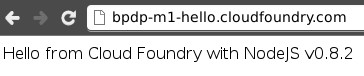
\includegraphics[scale=0.5]{images/modul1-hello-ganti-runtime.jpg}
    \end{center}
    \caption{Deployement menggunakan versi runtime tertentu}
    \label{fig:modul1-hello-ganti-runtime}
  \end{figure}

\subsection{Tanpa Framework}

Tanpa \textit{framework}, yang kita perlukan hanyalah langsung mem-\textit{push} file yang kita buat (dalam contoh ini adalah app.js):

\lstset{language=Javascript,caption=app.js tanpa framework}
\begin{lstlisting}

var http = require('http'); 
var url = require("url"); 

http.createServer(function (req, res) { 

    var pathname = url.parse(req.url).pathname; 

    res.writeHead(200, {'Content-Type': 'text/html'}); 
    res.write("Hello NodeJS <u>" + process.version + "</u>"); 
    res.write("<br />Request for <b>" + pathname + "</b> received."); 
    res.end(); 

}).listen(1337);
\end{lstlisting}

Proses deployement adalah sebagai berikut:

\lstset{language=bash,caption=Deployment app.js tanpa framework}
\begin{lstlisting}
$ vmc push --runtime=node08 
Would you like to deploy from the current directory? [Yn]: Y 
Application Name: bpdp-m1-hellonoframework 
Detected a Node.js Application, is this correct? [Yn]: Y 
Application Deployed URL [bpdp-m1-hellonoframework.cloudfoundry.com]: 
Memory reservation (128M, 256M, 512M, 1G, 2G) [64M]: 
How many instances? [1]: 
Create services to bind to 'bpdp-m1-hellonoframework'? [yN]: N 
Would you like to save this configuration? [yN]: N 
Creating Application: OK 
Uploading Application: 
  Checking for available resources: OK 
  Packing application: OK 
  Uploading (0K): OK   
Push Status: OK 
Staging Application 'bpdp-m1-hellonoframework': OK                              
Starting Application 'bpdp-m1-hellonoframework': OK                             

$
\end{lstlisting}

Hasilnya bisa dilihat pada Gambar~\ref{fig:modul1-hello-no-framework}

  \begin{figure}
    \begin{center}
      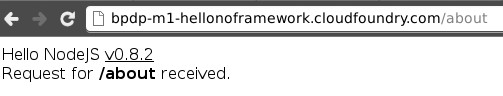
\includegraphics[scale=0.5]{images/modul1-hello-no-framework}
    \end{center}
    \caption{Hasil deployement app.js tanpa framework}
    \label{fig:modul1-hello-no-framework}
  \end{figure}
